\documentclass{article}
%\VignetteIndexEntry{IsotopeR}
\usepackage[utf8]{inputenc} % for UTF-8/single quotes from sQuote()
\usepackage{graphicx}
\usepackage{color}
\usepackage[colorlinks=true,urlcolor=blue,bookmarks=true]{hyperref}
\usepackage{url}
\author{Jack Hopkins \& Jake Ferguson}
\title{Estimating Diet Contributions with IsotopeR}
\newcommand{\code}[1]{{\tt #1}}
\date{\today}
\usepackage{Sweave}
\begin{document}
\maketitle
\tableofcontents



\code{IsotopeR} is a stable isotope mixing model used to estimate dietary parameters at the population- and individual-level. IsotopeR includes all features common to such analyses. We intended to make the IsotopeR user interface as simple and intuitive as possible and would welcome any feedback to continue to refine its user-friendliness. An example folder with data files for IsotopeR is available at \url{http://people.biology.ufl.edu/troutinthemilk/R_software_files/IsotopeR_Data.zip}.

\begin{figure}[h]
\begin{center}
  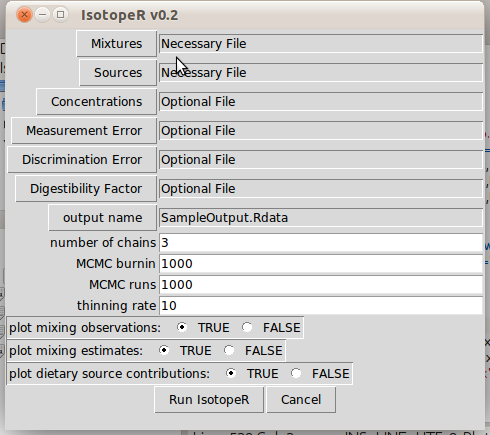
\includegraphics[width=0.5\textwidth]{IsoScreen.png}
\end{center}
\caption{The IsotopeR gui.}
\end{figure}


\section*{Installing and using IsotopeR:}

\begin{itemize}
\item Install JAGS from \url{http://sourceforge.net/projects/mcmc-jags/} (IsotopeR has been tested on JAGS v2.2.0, 2.1.0 and 1.0.4 under R 2.12 and 2.13)
\item  Install IsotopeR and its dependencies (tools, coda, lattice, runjags. ellipse, plotrix, fgui) from your favorite CRAN repository. You can then load and run the package with the following R code:
\begin{verbatim}
library(IsotopeR)
IsotopeR()
\end{verbatim}
If everything is correctly installed, once this code is run a window resembling illustration 1 will pop up.
	note: If using a Mac you will also need to install  the tcltk software from: \url{http://cran.r-project.org/bin/macosx/tools/}
\item  Setup data input files (described below) in the same format as the example data. Each data file name can be modified,  and all input files must be saved as .csv files, not .xls files.
\end{itemize}

\section*{Input files}

\textbf{Mixtures}: The first n columns in this data input file are the isotope values associated with each individual (i.e., consumer), where n is the number of isotopes used in the analysis. The last two columns designate the group and individual assignments. If there is no group structure, then column n + 1 will contain “1” for all individuals. If designating multiple groups, the group identity will be determined by the variable in the column. Individuals in the first group should be designated as “1,” the second group as “2,” etc. The last column identifies each individual. If you have no repeated measurements for individuals, then each individual should be designated by a unique integer (e.g., 1, 2, 3…); individuals with repeated measures should be designated using the same number (e.g., 1, 1, 1, 2, 2, 2…). 

Example:
\begin{center}
\begin{tabular}{llll}
$\delta$ X & $\delta$Y & group & individual\\
-21.11 & 5.82 & 1 & 1\\
-21.80 & 4.25 & 1 & 2\\
-21.03 & 4.72 & 1 & 3
\end{tabular}
\end{center}

\textbf{Source}: Each source is a sample of a consumer’s dietary items (may be a sample of the same species or an aggregate of species). The first n columns in this data input file are the isotope values associated with each sampled dietary item, where n is the number of isotopes used in the analysis. Isotope values need to be in the same order as the mixture data file (e.g., column 1 in Mixtures and Sources contain d13C values). The next column (i.e., n + 1) identifies the source to which the sampled dietary item belongs. The last column (subsource) identifies different species or taxa within each source aggregate; this feature assigns equal weight to each subsource. 

Example:
\begin{center}
\begin{tabular}{llll}
$\delta$X & $\delta$Y & source & subsource\\
-22.2 & 2.9 & plants & 1\\
-22.6 & 2.9 & plants & 1\\
-21.9 & 2.7 & plants & 1\\
-21.7 & 2.6 & plants & 2\\
-21.2 & 3.4 & plants & 2\\
-21.4 & 3.7 & animals & 1\\
-21.80 & 4.25 & animals & 1\\
\end{tabular}
\end{center}

\textbf{SourceCD}: The first n columns in this data input file are the concentration data for each sample, where n is the number of elemental concentrations used in the analysis (e.g., [C], [N]). Columns with elemental concentrations need to match Sources and Mixtures (e.g., column 1 in this file and Sources files contain [C] and d13C values, respectively). Column n + 1 identifies the source in which the set of concentrations belong. The last column links sampled dietary item concentrations to each subsource. This feature assigns equal weight to each sub-source’s elemental concentrations and should be consistent with Sources file.

Example:
\begin{center}
\begin{tabular}{llll}
[X] & [Y] & source & subsource\\
45 & 5 & plants & 1\\
46 & 5 & plants & 1\\
42 & 6 & plants & 1\\
42 & 4 & plants & 2\\
45 & 5 & plants & 2\\
10 & 3 & animals & 1\\
9 & 2 & animals & 1\\
\end{tabular}
\end{center}


\textbf{Measurement Error}: (error associated with mass spectrometry) This data input file contains all isotopic measurements for standards. Isotope values need to be in the same order as other data files (e.g., column 1 in MeasurementError, Mixtures, and Sources files contain d13C values). 

Example:
\begin{center}
\begin{tabular}{ll}
$\delta$X & $\delta$Y \\
-12.7 & 5.7\\
-12.6 & 5.9\\
-12.9 & 5.7\\
-12.7 & 5.6\\
\end{tabular}
\end{center}

\textbf{DiscrimSD}: (discrimination data) This data input file contains the standard deviations associated with the estimated discrimination factors measured in controlled diet studies. The first n columns are the standard deviations associated with each mean discrimination value for the associated isotope. The total discrimination variation.

Example:
\begin{center}
\begin{tabular}{ll}
$\delta$X & $\delta$Y \\
10.1 & 5.7\\
12.6 & 5.9\\
10.9 & 5.7\\
11.7 & 5.6\\
\end{tabular}
\end{center}


\textbf{Digest}: (digestibility corrections) This data file contains the digestibility of different sources. The first n columns contain the digestibility for n source isotopes. The next column is the source identification code defined in Sources. 

Example:
\begin{center}
\begin{tabular}{llll}
digestX & digestY & source\\
1 & .52 & plants \\
1 & .47 & animals & 1\\
\end{tabular}
\end{center}


\section*{Control Parameters}
The user can change the control parameters (defined below) for an MCMC run.
\begin{itemize}
 \item[Number of chains] The number of independent markov chains to be run.
 \item[MCMC burnin] The length of the chain discarded at the beginning of the run. This is interpreted as the length of time it takes for the MCMC to stabilize.
  \item[MCMC runs] The total number of iterations run per chain (includes burnin).
  \item[Thinning rate] Reduces the sample size to every nth iteration; this is used to reduce autocorrelation in the chain.
\end{itemize}


\section*{Output}
Plots
\begin{itemize}
	\item[Plot mixing observations] A plot of the mixing space (the estimated source means and the associated 95\% CI's) along with the mixture observations. If the measurement error data is provided the estimated 95\% CI's of the observation error will be displayed.
	\item[Plot mixing estimates] A plot of the mixing space (the estimated source means and the associated 95\% CI's)along with the estimated mixture values and the corresponding estimated 95\% CI's.
	\item[Plot dietary source contributions] A plot of the smoothed histograms of the population-level (black), group-level (red), and individual-level (blue) dietary estimates.
\end{itemize}

Results will be saved to an image file, \code{.Rdata} file and a text file, \code{.txt} (name of the file determined by output name field). Files can then be imported as a .csv file into Excel or OpenOffice. Files are formatted in a matrix with rows given by the parameter names (defined in table below). The first two columns are the mean and standard deviation of the posterior probability distribution. Quantiles (2.5\%, 25\%, 50\%, 75\%, 97.5\%) for this sampling distribution are reported in the following columns, followed by the Rhat values (a metric of convergence that should be less than 1.2 or the model should be rerun with a longer MCMC chain).


\section*{Estimated IsotopeR output parameters and definitions}


\begin{center}
\begin{tabular}{ll}
Parameter & Definition \\
mu.conc[y,z] & Mean concentration for element y, source z.\\
mu.mix[x,z] & Isotopic mixture value for individual x, source z (note: these are joint estimation values that include all sources of error).\\
mu.source[y,z] & Mean isotope value for isotope y, source z.\\
p[x,z] & Individual-level proportional dietary contribution for individual x, source z.\\
p.pop[x,z] & Population-level proportional dietary contribution for individual x, source z.\\
rho.source[z] & Correlation values between isotopes in source z.\\
sd.conc[i, z] & Concentration standard deviations for concentrations i and source z.\\
sd.me[i,z] & Measurement error standard deviations for isotope i and source z.\\
sd.res [i,j] & Standard deviations of the residual error term.\\
sd.source[i,z] & Source standard deviation for isotope i and source z.
\end{tabular}
\end{center}

A user may receive several warnings during a model run. These errors are associated with JAGS and are not well documented by the package maintainers. Generally, these errors are related to the model not converging. Therefore, you may need to rerun the model with more runs chains (and may also need a higher thinning rate).

Further details on the JAGS program can be found in the JAGS manual and available for download at \url{http://sourceforge.net/projects/mcmc-jags/}. A gentle introduction is provided in 'An Ecological Modeler's Primer on JAGS'. JAGS model syntax is compatible with the BUGS language. Users unfamiliar with the BUGS language can find many tutorials at the WinBUGS site \url{http://www.mrc-bsu.cam.ac.uk/bugs/}.


\end{document}
